% Created 2023-05-30 Tue 10:52
% Intended LaTeX compiler: pdflatex
\documentclass[11pt]{article}
\usepackage[utf8]{inputenc}
\usepackage[T1]{fontenc}
\usepackage{graphicx}
\usepackage{longtable}
\usepackage{wrapfig}
\usepackage{rotating}
\usepackage[normalem]{ulem}
\usepackage{amsmath}
\usepackage{amssymb}
\usepackage{capt-of}
\usepackage{hyperref}
\graphicspath{{../../books/}}
% TIPS
% \substack{a\\b} for multiple lines text





% pdfplots will load xolor automatically without option
\usepackage[dvipsnames]{xcolor}

\usepackage{forest}
% two-line text in node by [two \\ lines]
% \begin{forest} qtree, [..] \end{forest}
\forestset{
  qtree/.style={
    baseline,
    for tree={
      parent anchor=south,
      child anchor=north,
      align=center,
      inner sep=1pt,
    }}}
%\usepackage{flexisym}
% load order of mathtools and mathabx, otherwise conflict overbrace

\usepackage{mathtools}
%\usepackage{fourier}
\usepackage{pgfplots}
\usepackage{amsthm, mathabx,  amsmath, commath}
\usepackage{amsfonts}

\usepackage{empheq}
\usepackage{tikz}
\usetikzlibrary{arrows.meta}
\usepackage[most]{tcolorbox}

\newtheorem{theorem}{Theorem}[section]
\newtheorem{definition}{Definition}[section]
\newtheorem{corollary}{Corollary}[section]
\newtheorem{example}{Example}[section]
\newtheorem{lemma}{Lemma}[section]
\newtheorem{proposition}{Proposition}[section]

\newcommand{\bl}[1] {\boldsymbol{#1}}
\newcommand{\Wt}[1] {\stackrel{\sim}{\smash{#1}\rule{0pt}{1.1ex}}}
\newcommand{\wt}[1] {\widetilde{#1}}


%For boxed texts in align, use Aboxed{}
%otherwise use boxed{}

\DeclareMathSymbol{\widehatsym}{\mathord}{largesymbols}{"62}
\newcommand\lowerwidehatsym{%
  \text{\smash{\raisebox{-1.3ex}{%
    $\widehatsym$}}}}
\newcommand\fixwidehat[1]{%
  \mathchoice
    {\accentset{\displaystyle\lowerwidehatsym}{#1}}
    {\accentset{\textstyle\lowerwidehatsym}{#1}}
    {\accentset{\scriptstyle\lowerwidehatsym}{#1}}
    {\accentset{\scriptscriptstyle\lowerwidehatsym}{#1}}
}

\usepackage{graphicx}
    
% text on arrow for xRightarrow
\makeatletter
%\newcommand{\xRightarrow}[2][]{\ext@arrow 0359\Rightarrowfill@{#1}{#2}}
\makeatother


\def \bx {\boldsymbol{x}}
\def \ba {\boldsymbol{a}}
\def \bI {\boldsymbol{I}}
\def \bt {\boldsymbol{t}}
\def \bb {\boldsymbol{b}}
\def \bA {\boldsymbol{A}}
\def \bX {\boldsymbol{X}}
\def \bu {\boldsymbol{u}}
\def \bS {\boldsymbol{S}}
\def \bZ {\boldsymbol{Z}}
\def \bz {\boldsymbol{z}}
\def \by {\boldsymbol{y}}
\def \bw {\boldsymbol{w}}
\def \bT {\boldsymbol{T}}
\def \bS {\boldsymbol{S}}
\def \bm {\boldsymbol{m}}
\def \bW {\boldsymbol{W}}
\def \bY {\boldsymbol{Y}}
\def \bH {\boldsymbol{H}}
\def \blambda {\boldsymbol{\lambda}}
\def \bPhi {\boldsymbol{\Phi}}
\def \btheta {\boldsymbol{\theta}}
\def \bmu {\boldsymbol{\mu}}
\def \bphi {\boldsymbol{\phi}}
\def \bSigma {\boldsymbol{\Sigma}}
\def \lb {\left\{}
\def \rb {\right\}}
\def \caln {\mathcal{N}}
\def \dissum {\displaystyle\Sigma}
\def \dispro {\displaystyle\prod}
\def \E {\mathbb{E}}
\def \Q {\mathbb{Q}}
\def \V {\mathbb{V}}
\def \R {\mathbb{R}}
\def \calq {\mathcal{Q}}
\def \calg {\mathcal{G}}
\def \caln {\mathcal{N}}
\def \calr {\mathcal{R}}
\def \calm {\mathcal{M}}
\def \calc {\mathcal{C}}
\def \bcup {\bigcup}

\makeindex
\author{wu}
\date{\today}
\title{Big DataBase}
\hypersetup{
 pdfauthor={wu},
 pdftitle={Big DataBase},
 pdfkeywords={},
 pdfsubject={},
 pdfcreator={Emacs 29.0.90 (Org mode 9.6.1)}, 
 pdflang={English}}
\begin{document}

\maketitle
\tableofcontents

\section{Query Optimization}
\label{sec:org6ac77ef}
\subsection{Introduction}
\label{sec:org820094c}
Compile time system:
\begin{enumerate}
\item parsing: parsing, AST production
\item semantic analysis: schema lookup, variable binding, type inference
\item normalization, factorization, constant folding
\item rewrite 1: view resolution, unnesting, deriving predicates
\item plan generation: constructing the execution plan
\item rewrite 2: refining the plan, pushing group
\item code generation: producing the imperative plan
\end{enumerate}


Different optimization goals:
\begin{itemize}
\item minimize response time
\item minimize resource consumption
\item minimize time to first tuple
\item maximize throughput
\end{itemize}

Notation:
\begin{itemize}
\item \(\cala(e)\): attributes of the tuples produces by \(e\)
\item \(\calf(e)\) free variable of the expression \(e\)
\item binary operators \(e_1\theta e_2\) usually require \(\cala(e_1)=\cala(e_2)\)
\item \(\rho_{a\to b(e)}\), rename
\item \(\Pi_A(e)\), projection
\item \(\sigma_p(e)\), selection, \(\{x\mid x\in e\wedge p(x)\}\)
\item \(e_1\bowtie_pe_2\), join, \(\{x\circ y\mid x\in e_1\wedge y\in e_2\wedge p(x\circ y)\}\)
\end{itemize}

\subsection{Join Ordering}
\label{sec:org2ecd2b7}

\subsection{Accessing the Data}
\label{sec:org53f4ca7}

\subsection{Physical Properties}
\label{sec:org43a7943}

\subsection{Query Rewriting}
\label{sec:orgcb55afa}

\subsection{Self Tuning}
\label{sec:org4b8d456}
\section{Transaction System}
\label{sec:orge9e30a6}
\subsection{Computational Models}
\label{sec:orgfffb96c}
\subsubsection{Page Model}
\label{sec:org12c0203}
\begin{definition}[Page Model Transaction]
A \textbf{transaction} \(t\) is a partial order of steps of the form \(r(x)\) or \(w(x)\)
where \(x\in D\) and reads and writes as well as multiple writes applied to the same object are
ordered. We write \(t=(op,<)\) for transaction \(t\) with step set \(op\) and partial order \(<\)
\end{definition}
\subsubsection{Object Model}
\label{sec:orgdc0e4a0}
\begin{definition}[Object Model Transaction]
A \textbf{transaction} \(t\) is a (finite) tree of labeled nodes with
\begin{itemize}
\item the transaction identifier as the label of the root node,
\item the names and parameters of invoked operations as labels of inner nodes, and
\item page-model read/write operations as labels of leafs nodes, along with a partial order < on the
leaf nodes s.t. for all leaf-node operations \(p\) and \(q\) with \(p\) of the form \(w(x)\)
and \(q\) of the form \(r(x)\) or \(w(x)\) or vice versa, we have \(p<q\vee q<p\).
\end{itemize}
\end{definition}

\begin{center}
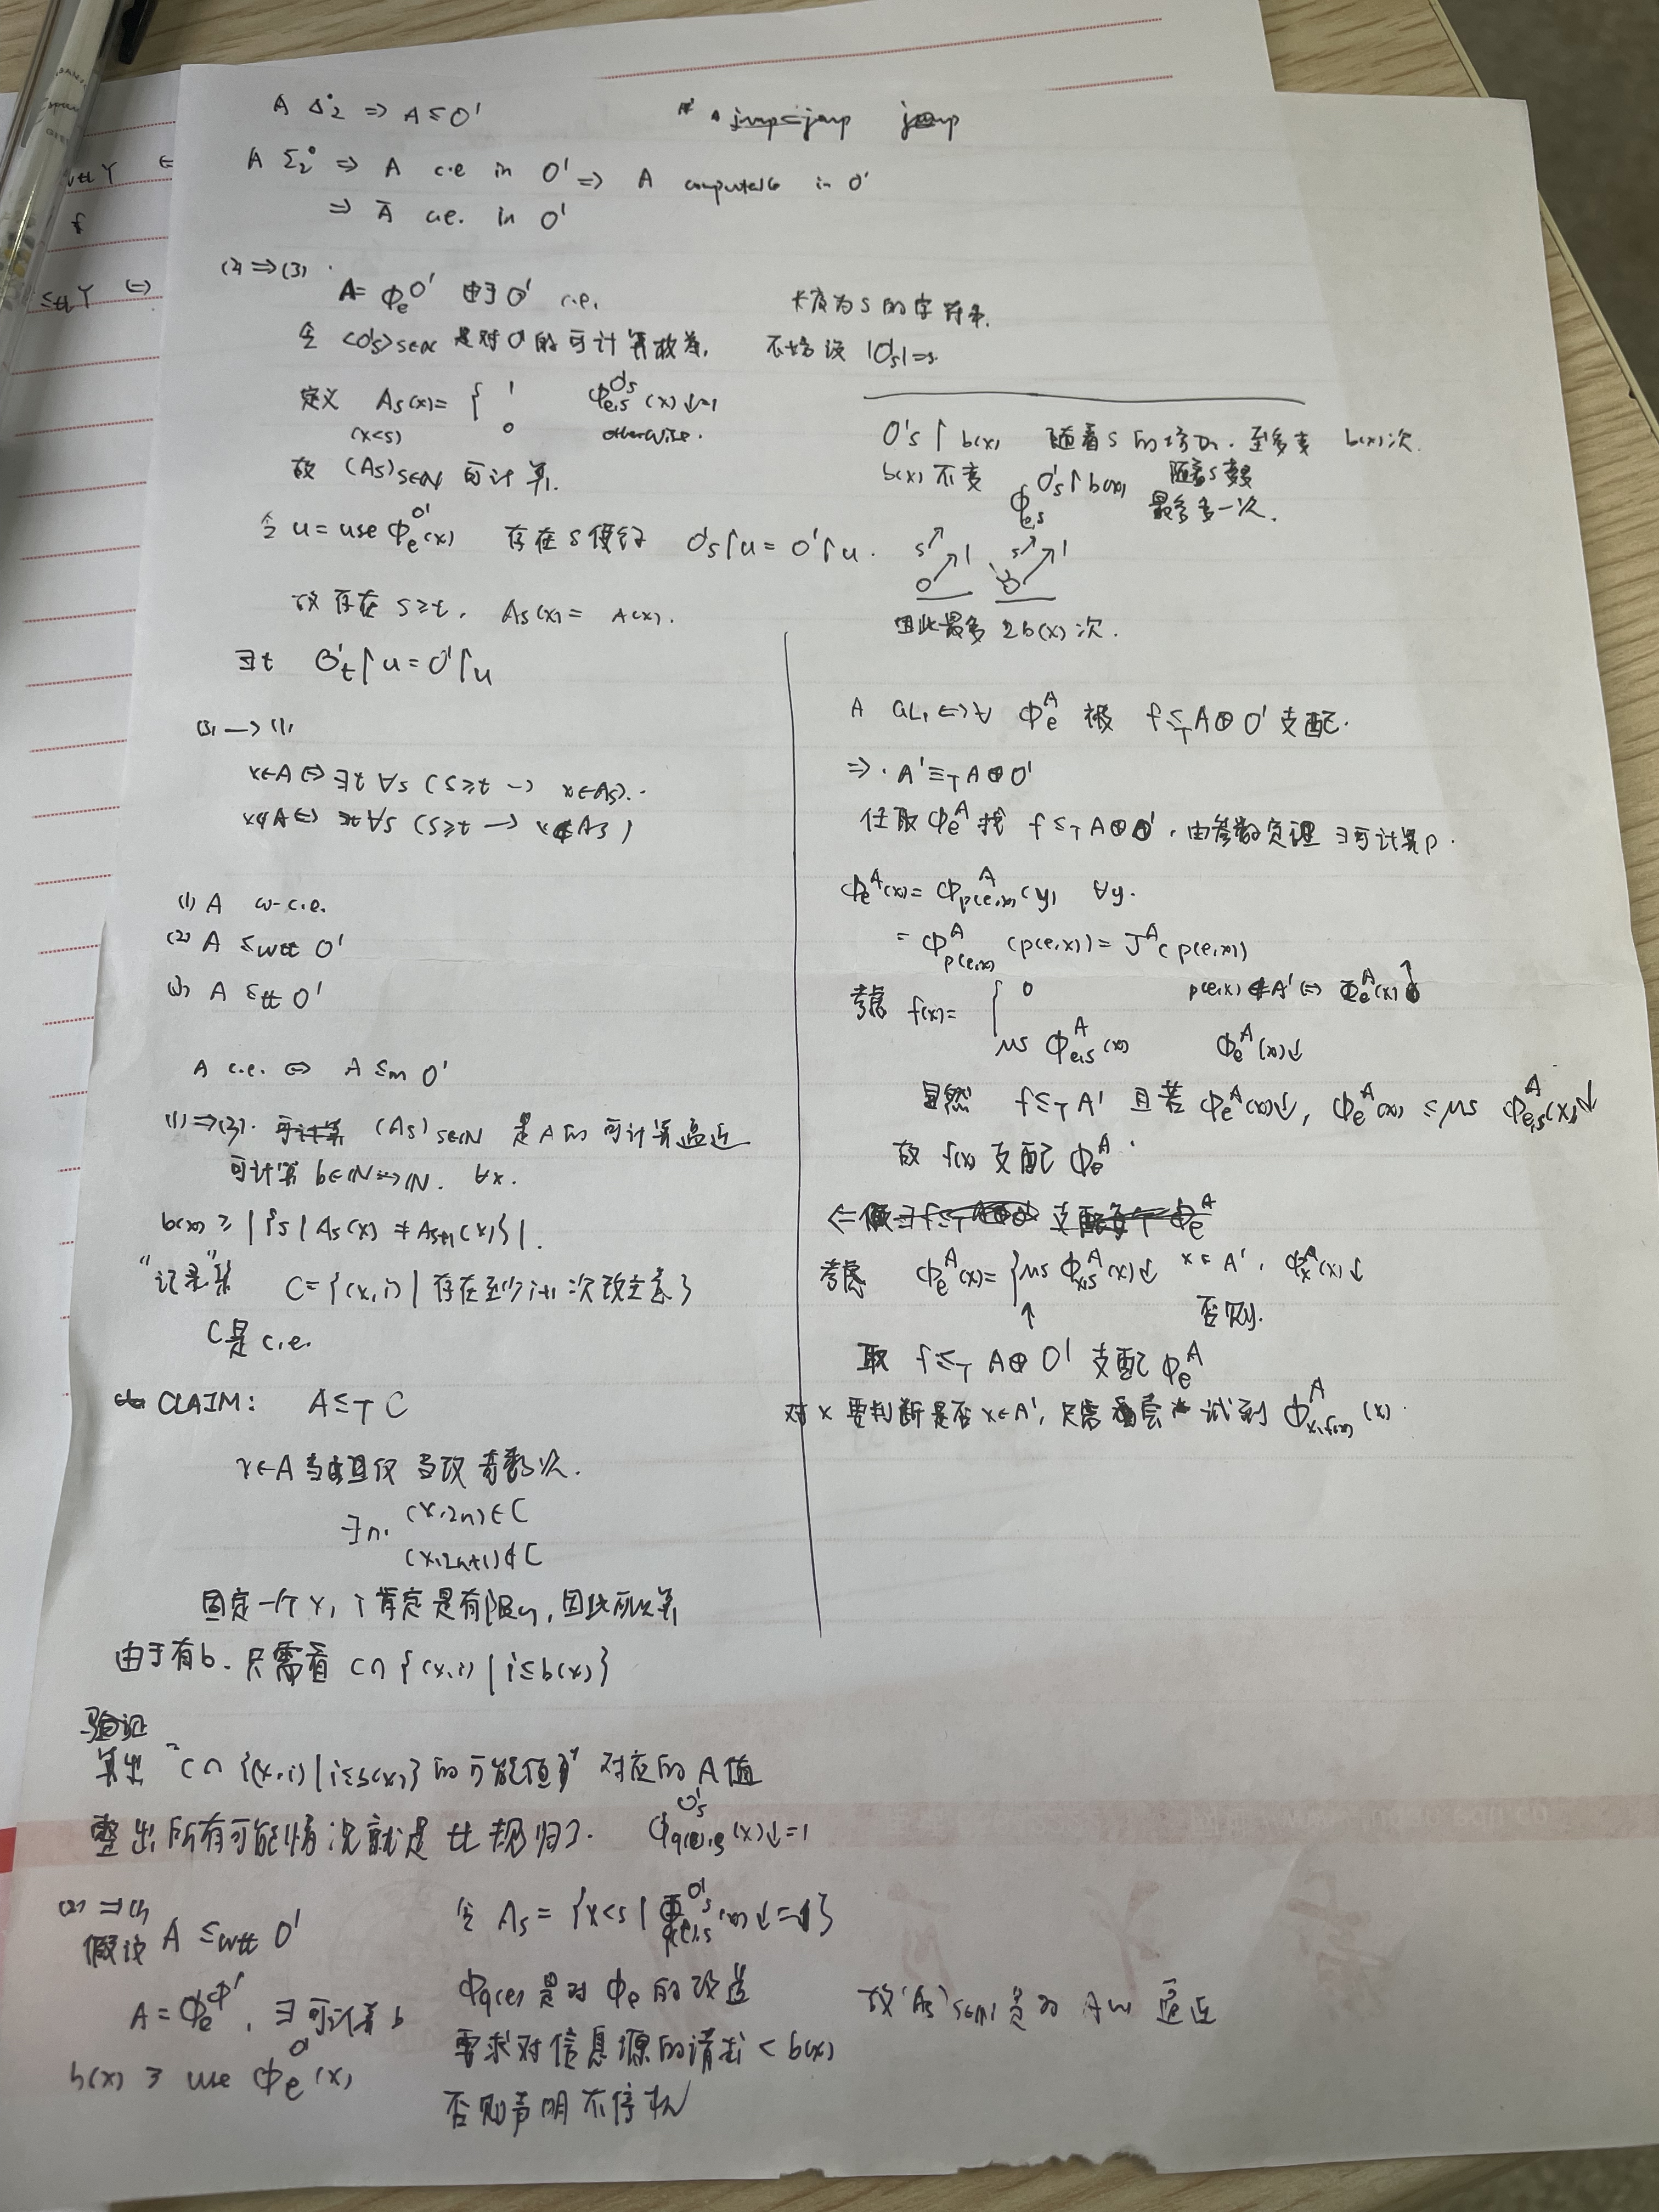
\includegraphics[width=.8\textwidth]{../images/bigdatabase/1.png}
\label{}
\end{center}
\subsection{Notions of Correctness for the Page Model}
\label{sec:orgdc6df74}
\subsubsection{Canonical Synchronization Problems}
\label{sec:org838a2f2}

Lost Update Problem:
\begin{center}
\includegraphics[width=.8\textwidth]{../images/bigdatabase/2.png}
\label{}
\end{center}

Inconsistent Read Problem
\begin{center}
\includegraphics[width=.8\textwidth]{../images/bigdatabase/3.png}
\label{}
\end{center}

Dirty Read Problem
\begin{center}
\includegraphics[width=.8\textwidth]{../images/bigdatabase/4.png}
\label{}
\end{center}
\subsubsection{Syntax of Histories and Schedules}
\label{sec:orge0a8247}
\begin{definition}[Schedules and histories]
Let \(T=\{t_1,\dots,t_n\}\) be a set of transactions, where each \(t_i\in T\) has the form
\(t_i=(op_i,<_i)\)
\begin{enumerate}
\item A \textbf{history} for \(T\) is a pair \(s=(op(s),<_s)\) s.t.
\begin{enumerate}
\item \(op(s)\subseteq\bigcup_{i=1}^nop_i\cup\bigcup_{i=1}^n\{a_i,c_i\}\)
\item for all \(1\le i\le n\), \(c_i\in op(s)\Leftrightarrow a_i\notin op(s)\)
\item \(\bigcup_{i=1}^n<_i\subseteq<_s\)
\item for all \(1\le i\le n\) and all \(p\in op_i\), \(p<_sc_i\vee p<_sa_i\)
\item for all \(p,q\in op(s)\) s.t. at least one of them is a write and both access the same
data item: \(p<_sq\vee q<_sp\)
\end{enumerate}
\item A \textbf{schedule} is a prefix of a history
\end{enumerate}
\end{definition}

\begin{definition}[]
A history \(s\) is \textbf{serial} if for any two transactions \(t_i\) and \(t_j\) in \(s\),
where \(i\neq j\), all operations from \(t_i\) are ordered in \(s\) before all operations
from \(t_j\) or vice versa
\end{definition}

\begin{center}
\includegraphics[width=.8\textwidth]{../images/bigdatabase/6.png}
\label{}
\end{center}

\begin{center}
\includegraphics[width=.8\textwidth]{../images/bigdatabase/5.png}
\label{}
\end{center}
\subsubsection{Herbrand Semantics of Schedules}
\label{sec:org23db092}
\begin{definition}[Herbrand Semantics of Steps]
For schedule \(s\) the \textbf{Herbrand semantics} \(H_s\) of steps \(r_i(x),w_i(x)\in op(s)\) is :
\begin{enumerate}
\item \(H_s[r_i(x)]:=H_s[w_j(x)]\) where \(w_j(x)\) is the last write on \(x\) in \(s\)
before \(r_i(x)\)
\item \(H_s[w_i(x)]:=f_{ix}(H_x[r_i(y_1)],\dots,H_s[r_i(y_m)])\) where
the \(r_i(y_j)\), \(1\le j\le m\), are all read operations of \(t_i\) that occur in \(s\)
before \(w_i(x)\) and \(f_{ix}\) is an uninterpreted \(m\)-ary function symbol.
\end{enumerate}
\end{definition}

\begin{definition}[Herbrand Universe]
For data items \(D=\{x,y,z,\dots\}\) and transactions \(t_i\), \(1\le i\le n\), the \textbf{Herbrand
universe HU} is hte smallest set of symbols s.t.
\begin{enumerate}
\item \(f_{0x}()\in HU\) for each \(x\in D\) where \(f_{0x}\) is a constant, and
\item if \(w_i(x)\in op_i\) for some \(t_i\), there are \(m\) read
operations \(r_i(y_1),\dots,r_i(y_m)\) that precede \(w_i(x)\) in \(t_i\),
and \(v_1,\dots,v_m\in HU\), then \(f_{ix}(v_1,\dots,v_m)\in HU\)
\end{enumerate}
\end{definition}

\begin{definition}[Schedule Semantics]
The \textbf{Herbrand semantics of a schedule} \(s\) is the mapping \(H[s]:D\to HU\) defined
by \(H[s](x):=H_s[w_i(x)]\) where \(w_i(x)\) is the last operation from \(s\) writing \(x\), for
each \(x\in D\)
\end{definition}

\begin{center}
\includegraphics[width=.6\textwidth]{../images/bigdatabase/7.png}
\label{}
\end{center}
\subsubsection{Final-State Serializability}
\label{sec:org4790b6a}
\begin{definition}[]
Schedules \(s\) and \(s'\) are called \textbf{final state equivalent}, denoted \(s\approx_fs'\)
if \(op(s)=op(s')\) and \(H[s]=H[s']\)
\end{definition}

\begin{definition}[Reads-from Relation]
Given a schedule \(s\), extended with an initial and a final transaction, \(t_0\)
and \(t_\infty\)
\begin{enumerate}
\item \(r_j(x)\) \textbf{reads \(x\) in \(s\) from \(w_i(x)\)} if \(w_i(x)\) is the last write on \(x\)
s.t. \(w_i(x)<_sr_j(x)\)
\item The \textbf{reads-from relation} of \(x\) is
\begin{equation*}
RF(s):=\{(t_i,x,t_j)\mid \text{an }r_j(x)\text{ reads \(x\) from a }w_i(x)\}
\end{equation*}
\item Step \(p\) is \textbf{directly useful} for step \(q\), denoted \(p\to q\), if \(q\) reads from \(p\),
or \(p\) is a read step and \(q\) is a subsequent write step of the same
transaction. \(\to^*\), the \textbf{useful relation}, denotes the reflexive and transitive closure of \(\to\).
\item Step \(p\) is \textbf{alive} in \(s\) if it is useful for some step from \(t_\infty\) and \textbf{dead}
otherwise
\item The \textbf{live-reads-from relation} of \(s\) is
\begin{equation*}
LRF(s):=\{(t_i,x,t_j)\mid \text{an alive \(r_j(x)\) reads \(x\) from \(w_i(x)\)}\}
\end{equation*}
\end{enumerate}
\end{definition}

\begin{theorem}[]
For schedules \(s\) and \(s'\) the following statements hold:
\begin{enumerate}
\item \(s\approx_fs'\) iff \(op(s)=op(s')\) and \(LRF(s)=LRF(s')\)
\item For \(s\) let the step graph \(D(s)=(V,E)\) be a directed graph with vertices \(V:=op(s)\)
and edges \(E:=\{(p,q)\mid p\to q\}\), and the reduced step graph \(D_1(s)\) be derived
from \(D(s)\) by removing all vertices that correspond to dead steps. Then \(LRF(s)=LRF(s')\)
iff \(D_1(s)=D_1(s')\)
\end{enumerate}
\end{theorem}

\begin{corollary}[]
Final-state equivalence of two schedules \(s\) and \(s'\) can be decided in time that is
polynomial in the length of the two schedules.
\end{corollary}
\subsubsection{View Serializability}
\label{sec:org10d71af}
As we have seen, FSR emphasizes steps that are alive in a schedule. However, since the semantics
of a schedule and of the transactions occurring in a schedule are unknown, it is reasonable to
require that in two equivalent schedules, each transaction reads the same values, independent of
its liveliness.

\textbf{Lost update anomaly}: \(L=r_1(x)r_2(x)w_1(x)w_2(x)c_1c_2\). History is not
FSR,
 \(LRF(L)=\{(t_0,x,t_2),(t_2,x,t_\infty)\}\),
 \(LRF(t_1t_2)=\{(t_0,x,t_1),(t_1,x,t_2),(t_2,x,t_\infty)\}\) and
 \(LRF(t_2t_1)=\{(t_0,x,t_2),(t_2,x,t_1),(t_1,x,t_\infty)\}\)


\textbf{Inconsistent read anomaly}: \(I=r_2(x)w_2(x)r_1(x)r_1(y)r_2(y)w_2(y)c_1c_2\), history is FSR
\(LFR(I)=LFR(t_1t_2)=LFR(t_2t_1)=\{(t_0,x,t_2),(t_0,y,t_2),(t_2,x,t_\infty),(t_2,y,t_\infty)\}\)


\begin{definition}[View Equivalence]
Schedules \(s\) and \(s'\) are \textbf{view equivalent}, denoted \(s\approx_vs'\), if the following
hold:
\begin{enumerate}
\item \(op(s)=op(s')\)
\item \(H[s]=H[s']\)
\item \(H_s[p]=H_{s'}[p]\) for all (read or write) steps
\end{enumerate}
\end{definition}

\begin{theorem}[]
For schedules \(s\) and \(s'\) the following statements hold.
\begin{enumerate}
\item \(s\approx_v s'\) iff \(op(s)=op(s')\) and \(RF(s)=RF(s')\)
\item \(s\approx_vs'\) iff \(D(s)=D(s')\)
\end{enumerate}
\end{theorem}

\begin{proof}
\begin{enumerate}
\item \(\Rightarrow\): Consider a read step \(r_i(x)\) from \(s\).
Then \(H_s[r_i(x)]=H_{s'}[r_i(x)]\) implies that if \(r_i(x)\) reads from some
step \(w_j(x)\) in \(s\), the same holds in \(s'\), and vice versa.

\(\Leftarrow\): If \(RF(s)=RF(s')\), this in particular applies to \(t_\infty\);
hence \(H[s]=H[s']\). Similarly, for all other reads \(r_i(x)\) in \(s\), we
have \(H_s[r_i(x)]=H_{s'}[r_i(x)]\).

Suppose for some \(w_i(x)\), \(H_s[w_i(x)]\neq H_{s'}[w_i(x)]\). Thus the set of values read
by \(t_i\) prior to step \(w_i\) is different in \(s\) and \(s'\), a contradiction to our
assumption that \(RF(s)=RF(s')\).
\end{enumerate}
\end{proof}

\begin{corollary}[]
View equivalence of two schedules \(s\) and \(s'\) can be decided in time that is polynomial in
the length of the two schedules
\end{corollary}

\begin{definition}[]
A schedule \(s\) is \textbf{view serializable} if there exists a serial schedule \(s'\)
s.t. \(s\approx_vs'\). VSR denotes the class of all view-serializable histories
\end{definition}

\begin{theorem}[]
\(VSR\subset FSR\)
\end{theorem}

\begin{theorem}[]
Let \(s\) be a history without dead steps. Then \(s\in VSR\) iff \(s\in FSR\)
\end{theorem}

\begin{theorem}[]
The problem of deciding for a given schedule \(s\) whether \(s\in VSR\) holds is NP-complete
\end{theorem}

\begin{definition}[Monotone Classes of Histories]
Let \(s\) be a schedule and \(T\subseteq trans(s)\). \(\pi_T(s)\) denotes the projection
of \(s\) onto \(T\). A class of histories is called \textbf{monotone} if the following holds:
\begin{center}
If \(s\) is in \(E\), then \(\Pi_T(s)\) is in \(E\) for each \(T\subseteq trans(s)\)
\end{center}
\end{definition}

VSR is not monotone
\subsubsection{Conflict Serializability}
\label{sec:org806ffb7}
\begin{definition}[Conflicts and Conflict Relations]
Let \(s\) be a schedule, \(t,t'\in trans(s)\), \(t\neq t'\)
\begin{enumerate}
\item Two data operations \(p\in t\) and \(q\in t'\) are in \textbf{conflict} in \(s\) if
they access the same data item and at least one of them is a write
\item \(conf(s):=\{(p,q)\mid p,q\text{ are in conflict and }p<_sq\}\) is the \textbf{conflict relation} of \(s\)
\end{enumerate}
\end{definition}

\begin{definition}[]
Schedules \(s\) and \(s'\) are \textbf{conflict equivalent}, denoted \(s\approx_cs'\),
if \(op(s)=op(s')\) and \(conf(s)=conf(s')\)
\end{definition}

\begin{definition}[]
Schedule \(s\) is \textbf{conflict serializable} if there is a serial schedule \(s'\)
s.t. \(s\approx_cs'\). CSR denotes the class of all conflict serializable schedules.
\end{definition}

\begin{theorem}[]
\(CSR\subset VSR\)
\end{theorem}

\begin{definition}[]
Let \(s\) be a schedule. The \textbf{conflict graph} \(G(s)=(V,E)\)  is a directed graph with
vertices \(V:=commit(s)\) and
edges \(E:=\{(t,t')\mid t\neq t'\text\wedge\exists p\in t,q\in t':(p,q)\in conf(s)\}\)
\end{definition}

\begin{theorem}[]
Let \(s\) be a schedule. Then \(s\in CSR\) iff \(G(s)\) is acyclic.
\end{theorem}

\begin{proof}
\(\Rightarrow\): There is a serial history \(s'\) s.t. \(op(s)=op(s')\)
and \(conf(s)=conf(s')\). Consider \(t,t'\in V\), \(t\neq t'\) with \((t,t')\in E\). Then we
have
\begin{equation*}
(\exists p\in t)(\exists q\in t')p<_sq\wedge(p,q)\in conf(s)
\end{equation*}
Then \(p<_{s'}q\). Also all of \(t\) occur before all of \(t'\) in \(s'\).

Suppose \(G(s)\) were cyclic. Then we have a cycle \(t_1\to t_2\to\dots\to t_k\to t_1\). The
same cycle also exists in \(G(s')\), a contradiction

\(\Leftarrow\):
\end{proof}

\begin{corollary}[]
Testing if a schedule is in CSR can be done in time polynomial to the schedule's number of transactions
\end{corollary}

Commutativity rules:
\begin{enumerate}
\item \(C_1:r_i(x)r_j(y)\sim r_j(y)r_i(x)\) if \(i\neq j\)
\item \(C_2:r_1(x)w_j(y)\sim w_j(y)r_i(x)\) if \(i\neq j\) and \(x\neq y\)
\item \(C_3:w_i(x)w_j(y)\sim w_j(y)w_i(x)\) if \(i\neq j\) and \(x\neq y\)
\end{enumerate}
Ordering rule:
\begin{enumerate}
\setcounter{enumi}{3}
\item \(C_4\): \(o_i(x)\), \(p_j(y)\) unordered \(\Rightarrow\) \(o_i(x)p_j(y)\)
if \(x\neq y\) or both \(o\) and \(p\) are reads
\end{enumerate}


\begin{definition}[]
Schedules \(s\) is \textbf{commit order preserving conflict serializable} if for
all \(t_i,t_j\in trans(s)\), if there are \(p\in t_i\), \(q\in t_j\) with \((p,q)\in conf(s)\),
then \(c_i<_sc_j\).

COCSR denotes the class of all schedules with this property
\end{definition}

\begin{theorem}[]
\(COCSR\subset CSR\)
\end{theorem}

\begin{theorem}[]
Schedule \(s\) is in COCSR iff there is a serial schedule \(s'\) s.t. \(s\approx_cs'\) and for
all \(t_i,t_j\in trans(s)\): \(t_i<_{s'}t_j\Leftarrow c_i<_{s}c_j\)
\end{theorem}
\subsubsection{An Alternative Criterion: Interleaving Specifications}
\label{sec:org60739c3}
\subsection{Concurrency Control Algorithms}
\label{sec:org81d9781}
\subsubsection{General Scheduler Design}
\label{sec:org7323902}
\begin{center}
\includegraphics[width=.8\textwidth]{../images/bigdatabase/8.png}
\label{}
\end{center}

\begin{definition}[CSR Safety]
For a scheduler \(S\), \(Gen(S)\) denotes the set of all schedules that \(S\) can generate. A
scheduler is called \textbf{CSR safe} if \(Gen(S)\subseteq CSR\)
\end{definition}
\begin{forest}
[concurrency control protocols
    [pessimistic
        [non-locking
            [TO]
            [SGT]
        ]
    ]
]
\end{forest}
\subsubsection{Locking Schedulers}
\label{sec:org4a9d132}
\subsubsection{Non-Locking Schedulers}
\label{sec:orgca01522}
\subsubsection{Hybrid Protocols}
\label{sec:org97079be}
\end{document}
